\section{Convergence vers le modèle de Black-Scholes}

Avant de continuer à étudier le modèle binomial, il est nécessaire de comprendre que le modèle de Cox-Ross-Rubinstein est une discrétisation d'un autre modèle que nous allons voir dans cette section : le modèle de \textbf{Black-Scholes}.

\subsection{Mouvement Brownien / Processus de Wiener}
Commençons par introduire un phénomène mathématique fort utile : le \textbf{mouvement brownien}, introduit en 1827 par le botaniste \textbf{Robert Brown}. Le mouvement brownien décrit le mouvement aléatoire d'une particule dans un fluide, subissant des chocs avec les autres particules du milieu. Entre deux chocs, la particule se déplace avec un mouvement rectiligne uniforme. La nature de ce procédé chaotique peut être modélisé à l'aide d'un processus stochastique appelé \textbf{Processus de Wiener}, utilisable pour la représentation d'une évolution de marché incertain. En 1933, le mathématicien Paul Lévy a démontré que le mouvement brownien est une martingale continue ce qui nous permettra d'utiliser les résultats évoqués dans les sections précédentes. On notera $W_t : \mathbb{\mathbb{R}^+} \to \mathbb{R}^d$ le processus de Wiener associé à un mouvement brownien à l'instant $t \in I$ dans un espace de dimension $d$. \\
\vspace{0.02\textheight}
\begin{definitionbox}[frametitle = {Processus de Wiener}]
    On dit qu'une famille de variables aléatoires réelles $(W_t)_{t \in \mathbb{R}^+}$ est un processus de Wiener si :
    \begin{itemize}
        \item $W_0 = 0$
        \item $\forall \omega \in \Omega,t \mapsto W_t(\omega)$ est continue
        \item $\forall t_0<t_1<...<t_n, \forall i \in \{1,...,n\}, \ \ W_0, W_{t_1} - W_{t_0}, ..., W_{t_n} - W_{t_{n-1}}$ sont \\ indépendantes 
        \item $\forall A \in \mathcal{B}(\mathbb{R}), \forall s,t \in \mathbb{R}^+, \mathbb{P}(W_{s+t} - W_s \in A) = \Large \int_A \frac{1}{{\sqrt{2 \pi t}}}e^{-\frac{x^2}{2t}}dx $
    \end{itemize}
\end{definitionbox}



\begin{figure}[H]
    \centering
    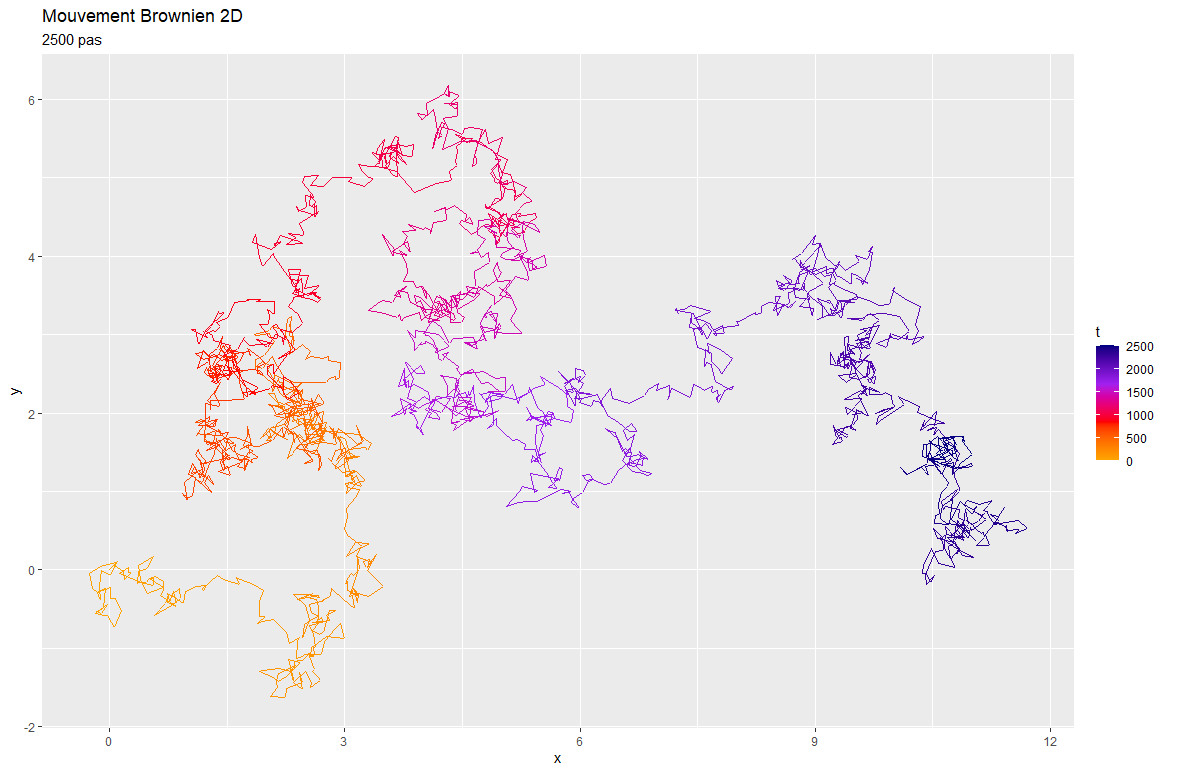
\includegraphics[width=1.1\textwidth]{Images/brownien2D.png}
    \caption{Simulation du mouvement Brownien 2D}
\end{figure}
\vspace{0.03\textheight}
\remarque Le processus de Wiener est continu partout mais dérivable nulle part. Il s'apparente en ce sens à une fonction de Weierstrass.
\vspace{0.025\textheight}\\
Si on considère le déplacement d'une particule dans un espace de dimension $d$, on peut alors associer l'évolution de sa position au processus de Wiener $W_t : \mathbb{\mathbb{R}^+} \to \mathbb{R}^d$. On obtient, de par la nature du mouvement brownien, que la distance moyenne parcourue par la particule jusqu'à $t_\alpha$ vaut $\mathbb{E}[W_t] = 0$ car le mouvement brownien n'a pas de direction privilégiée. \\
Ainsi, on remarque directement que $Var(W_t) = \mathbb{E}[W_t^2]-\mathbb{E}[W_t]^2 = \mathbb{E}[W_t^2]$. \\
On considèrera uniquement les mouvements browniens unidimensionnels par la suite.



On peut également montrer que $W_t$ est un cas particulier de processus stochastique gaussien, c'est-à-dire :
\begin{align*}
    \forall A \subset I, \ \forall (a_t)_{t\in A} \subset \mathbb{R}, \ \ \sum_{s \in A} a_s W_s \sim \mathcal{N}(\mu, \sigma^2) 
\end{align*}

Considérons une option sur un marché. A chaque instant $t$ son prix augmente ou baisse. On peut ainsi modéliser l'évolution du prix d'une option par une marche aléatoire. \\
D'après le \textbf{théorème de Donsker}, cette marche aléatoire converge en loi vers un mouvement brownien standard $W = (W_t, t \geq 0)$. Ainsi, étudier le caractère aléatoire et chaotique de l'évolution du prix d'une option revient à étudier un mouvement brownien.\\

\begin{figure}[H]
    \centering
    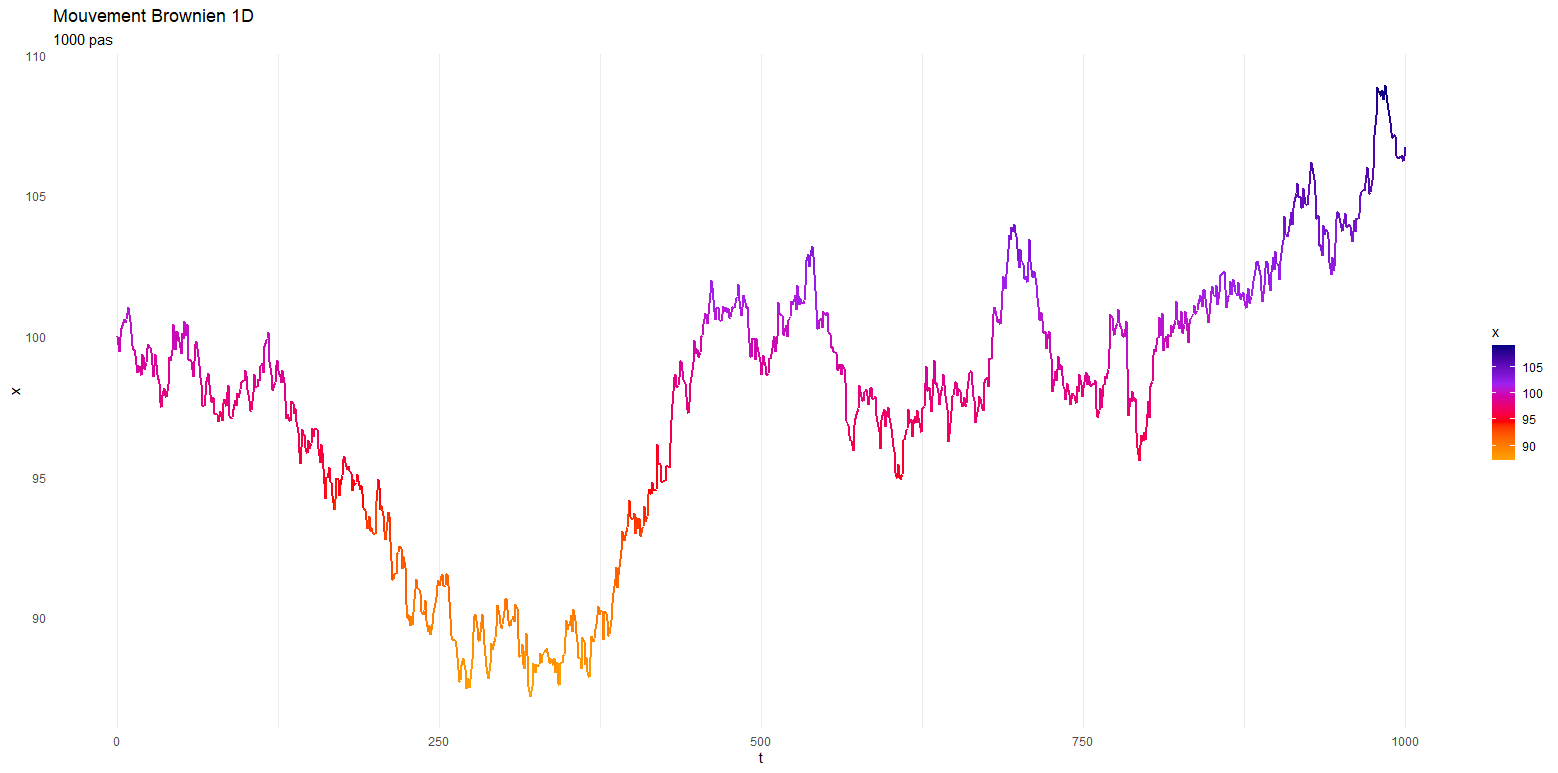
\includegraphics[width=1.1\textwidth]{Images/brownien1D.png}
    \caption{Simulation du mouvement Brownien 1D}
\end{figure}


\subsection{Intégration d'Itō}

Comme vu précédemment,  Il n'existe donc pas de dérivée au sens classique du terme. Le mathématicien Kiyoshi Itō a ainsi développé une nouvelle théorie de l'intégration reposant sur le caractère aléatoire des fonctions à étudier. On va maintenant s'intéresser au calcul des intégrales d'Itō. Ces intégrales permettent d'intégrer des variables aléatoires. L'intégrale est également une variable aléatoire et, en particulier, est une martingale.
\\


On considère un processus de Wiener $W_t$ sur un intervalle $I = [0; T]$ avec $T \in \mathbb{R^+}$ et une subdivision régulière de cet intervalle $0=t_0<t_1<...<t_n=T$, avec $n \in \mathbb{N}$. De manière analogue à l'intégration de Riemann, on peut approcher la valeur de l'intégrale à l'aide de sommes partielles de rectangles de longueur $t_{i+1}-t_i$ et de hauteur $W_t$. Le côté gauche du rectangle doit coïncider avec la valeur à gauche de l'intégrande car le mouvement brownien est une martingale et ne doit pas tenir compte du futur (si l'on prenait le milieu de chaque segment de subdivision, on obtiendrait une intégrale de Stratonovich). Ainsi l'intégrale d'Itō est définie comme la limite en moyenne quadratique de la somme de Riemann évaluée en borne gauche :

\begin{align*}
    I(T) = \int_0^T W_tdW_t &= \lim_{n \to \infty} \sum_{i=0}^{n-1} W_{t_i}(W_{t_{i+1}}-W_{t_i})\\
    \text{en utilisant l'identité }& a(b-a) = \frac{1}{2}(b^2-a^2-(b-a)^2) \text{ avec } a = W_{t_i} \text{ et } b = W_{t_{i+1}}\\
    \implies W_{t_i}(W_{t_{i+1}}-W_{t_i}) &= \frac{1}{2}(W_{t_{i+1}}^2-W_{t_i}^2)-\frac{1}{2}(W_{t_{i+1}}-W_{t_i})^2 \\
    \implies \sum_{i=0}^{n-1} W_{t_i}(W_{t_{i+1}}-W_{t_i}) &= \frac{1}{2}\sum_{i=0}^{n-1}(W_{t_{i+1}}^2-W_{t_i}^2)-\frac{1}{2}\sum_{i=0}^{n-1}(W_{t_{i+1}}-W_{t_i})^2 \\
    \text{or }\sum_{i=0}^{n-1} (W_{t_{i+1}}^2 - W_{t_i}^2) &= W_{t_n}^2 - W_{t_0}^2 = W_T^2 \text{ par somme téléscopique}\\
    \text{et }\sum_{i=0}^{n-1} (W_{t_{i+1}} - W_{t_i})&^2 \xrightarrow{L^2} T \text{ car } \mathbb{E}[(W_{t_{i+1}} - W_{t_i})^2] = Var(W_{t_{i+1}} - W_{t_i}) = t_{i+1} - t_i\\
    \implies I(T) &= \int_0^TW_tdW_t=\frac{1}{2}W_T^2-\frac{1}{2}T\\
\end{align*}

Ainsi, $I(t)$ dépend de deux membres, le premier représentant la position finale quadratique et le second correspond à un ajustement de la volatilité. Sans le dernier terme, l'intégrale ne serait pas une martingale.\\

Terminons notre introduction de ce type d'intégration avec un lemme appelé : \textbf{Lemme d'Itō}.
Il faut ainsi définir le \textbf{processus d'Itō :}
\
$$I_t = \int_0^t \mu_sds+\int_0^t\sigma_sdW_s \quad\text{ qui est équivalent à } \quad dI_t=\mu_tdt+\sigma_tdW_t$$
avec $W_t$ un processus de Wiener, $\mu\in L^1$ et $\sigma\in L^2$ des processus déterministes. \\
\remarque Le processus de Wiener a une espérance nulle donc $\mathbb{E}[I_t]=\int_0^t\mu_sds$ et a une variance non nulle donc $Var[X_t]=\int_0^t\sigma^2dW_s$ \\

\begin{definitionbox}[frametitle = {Lemme d'Itō}]
    Soit $\mu\in L^1$,$\sigma\in L^2$,$I_t$ un processus d'Itō et $f(I_t,t)$ une fonction de classe $\mathcal{C}^2(\mathbb{R \times R^+, R)}$ alors :
    $$d(f(I_t,t))=\dfrac{\partial f}{\partial t}(I_t,t)dt+\dfrac{\partial f}{\partial x}(I_t,t)dI_t+\frac{1}{2}\dfrac{\partial^2 f}{\partial x^2}(I_t,t)\sigma^2_tdt$$
\end{definitionbox}

On a précédemment comparé l'évolution d'une option sur un marché à un mouvement brownien. Cependant, le prix d'une option ne peut pas être négatif. Pour pallier ce problème, on peut définir le \textbf{processus log-normal} ou \textbf{mouvement brownien géométrique} :
$$X_t = X_0e^{(a-\frac{1}{2}\sigma^2)t + \sigma W_t} \quad\text{avec } a,\sigma\in \mathbb{R}$$
Ainsi, on le mouvement brownien géométrique est solution de l'équation différentielle stochastique : $dX_t = a X_t dt + \sigma X_t dW_t$ \\
\proofname{} \\
Soit $X_t = X_0e^{(a-\frac{1}{2}\sigma^2)t + \sigma W_t} \quad\text{avec } a,\sigma\in \mathbb{R}$. On pose alors le processus d'Itō $I_t = (a - \frac{1}{2}\sigma^2)t + \sigma W_t$. \\
On a alors $dY_t = \underbrace{(a - \frac{1}{2}\sigma^2)}_{\mu_t} dt + \underbrace{\sigma}_{\sigma_t} dW_t$ \\
On définit la fonction $f(x, t) = X_0 e^x$ telle que $f(I_t, t) = X_t$
\begin{itemize}
    \item $\dfrac{\partial f}{\partial t}(I_t, t)=0$
    \item $\dfrac{\partial f}{\partial x}(I_t, t)=X_0e^{I_t}=X_t$
    \item $\dfrac{\partial^2 f}{\partial x^2}(I_t, t)=X_0e^{I_t}=X_t$
\end{itemize}
On peut alors appliquer le lemme d'Itō:
$$dX_t = 0 \cdot dt + X_tdI_t+\dfrac{1}{2}X_t\sigma^2dt$$
Substituons $dI_t$ par $(a - \frac{1}{2}\sigma^2)dt + \sigma dW_t$ :
\begin{align*}
    dX_t &= X_t[(a - \frac{1}{2}\sigma^2)dt + \sigma dW_t]+\dfrac{1}{2}X_t\sigma^2dt \\
    &= aX_tdt - \frac{1}{2}\sigma^2X_tdt +\sigma X_tdW_t+\dfrac{1}{2}X_t\sigma^2dt \\
    &=aX_tdt+\sigma X_tdW_t
\end{align*}
Finalement, on a bien : 
$$dX_t = a X_t dt + \sigma X_t dW_t$$ \\

Après avoir défini tous ces processus, nous allons pouvoir les appliquer au modèle de Black-Scholes dans la sous-partie suivante.
\subsection{Equation de Black-Scholes}
Introduisons maintenant l'équation aux dérivées partielles la plus importante des mathématiques financières : l'équation de Black-Scholes dont le nom fait référence à Fischer Black et Myron Scholes qui l'ont évoqué dans un texte de recherche académique. Nous allons étudier le modèle de Black-Scholes dans un premier temps avant de montrer qu'en diminuant les pas de temps, le modèle de cox-Ross-Rubinstein converge vers le modèle de Black-Scholes.

\vspace{0.05\textheight}
\begin{definitionbox}[frametitle = {Equation aux Dérivées Partielles de Black-Scholes}]
    Soit $V(S,t)$ le prix d'une option avec $S$ le prix du sous-jacent et $t$ représentant le temps :
    $$\frac{\partial V}{\partial t} + \frac{1}{2}\sigma^2S^2\frac{\partial^2V}{\partial S^2}+rS\frac{\partial V}{\partial S}-rV=0$$
\end{definitionbox}
\vspace{0.05\textheight}
Le modèle repose sur un grand nombre d'hypothèses assez contraignantes, nécessaires pour la démonstration de la formule. Le but étant d'étudier le modèle de Cox-Ross-Rubinstein. Je vais donner les hypothèses simplifiées nécessaires à la compréhension de la résolution. Elles sont néanmois trouvables sur \hyperlink{https://fr.wikipedia.org/wiki/Modèle_Black-Scholes}{la page Wikipédia du modèle de Black-Scholes}. 
\vspace{0.025\textheight}\\
Les hypothèses de ce modèle sont donc : 
\begin{itemize}
    \item Le taux sans risque est constant
    \item Le prix suit un mouvement brownien géométrique et la variance du mouvement est constante
    \item L'option ne donne pas de dividende
    \item Le marché respecte l'AOA
    \item Le marché permet de vendre un actif en n'importe quelle quantité
    \item Les transactions n'occasionnent aucun frais
\end{itemize}
\vspace{0.025\textheight}
La formule de Black-Scholes permet de calculer le prix d'un \textbf{call ou put européen} mais ne permet pas de calculer des calls/puts américains contrairement au modèle de Cox-Ross-Rubinstein.

\subsection{Convergence}